\section{Number Representations}
\subsection{Types}
\paragraph{Base Two}
Numbers in computers are represented in binary, base two, format. Normally, our normal understanding of numbers is in Base Ten. \[3 = 1 \times 10^0\] but this can also be represented in Base Two \[3_10 = 11_2 = 1 \times 2^1 + 1 \times 2^0\]. In terms of integers at least, this means that the maximum size we can represent in $n$ bits is \[2^n - 1\] so a 32-bit value is, at most, $2^{32} - 1$.
\paragraph{Representations}
Ofcourse, this method of representation using twos also works for decimals, but where in a byte do we store decimals? In the fixed point representation of real numbers, the decimal is implied. For example, assuming a 16-bit piece of memory, we imply that the integer portion will cover the first 8 bits and the decimal portion the remaining 8 bits. As such, the computer will recognize the values with no manual decimal placed.
Modern computers now use the floating point representation. \[V = M \times 2^E\] Floating point uses a mantissa $M$ and an exponent $E$ to store its values. Part of the bits, for example 4 bits in an 8-bit system, are used to store the mantissa and the rest represent the exponent. In an 8 bit system as a result, you can represent a value like 112 as \[01110111 \rightarrow 0.111 \times 2^{0111}\]
\paragraph{Negative Value}
Negative values are represented using something we like to call Two's Complement. What this simply means is, the left-most bit is "0" for the positive variant. We know that each value we can represent should have a value in the same field that, when added together, form $0$. We represent this negative value by inverting every bit and adding 1 to the LSB. \[ 0101 \rightarrow 1011\]. The system reads the left-most bit as a 1, so we know its negative, the rest follows.

\subsection{Arithmetic}
\begin{figure}[!htb]
	\center{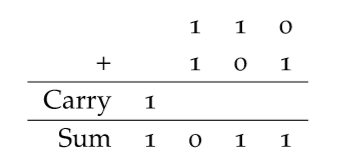
\includegraphics[width=5cm]
		{csa/adding}}
	\caption{\label{fig:adding} Arithmetic example for base 2}
\end{figure}
Adding bits works the same as adding and subtracting the numbers in base 10. For example, if we were to add $0110$ and $0101$, the result would be $1011$ as seen by the figure. When our column adds to a total of 2, a one is carried on column to the right and the 2 becomes a 0. If the total becomes 3, a 1 is still carried, but the column becomes a 1.
For subtraction, you can add the base value and the two's compliment of the other value. This simplifies the process greatly.

\section{Logic}
\subsection{Logic Gates}
The basic building block of our CPUs today are transistors. Transistors are made up of three parts, a gate, a source, and a drain. They are used in circuits; it is enough to understand that they are switches that are controlled by the gate voltage.
Transistors process bits (0 voltage and $>$ 0 voltage). The output changes based on how the circuit is built. For example, we have the NOT gate which takes a signal and inverts it on output. For simplicity, gates are drawn in an abbreviated form as seen in Figure \ref{fig:gates}.
\begin{figure}[!htb]
	\center{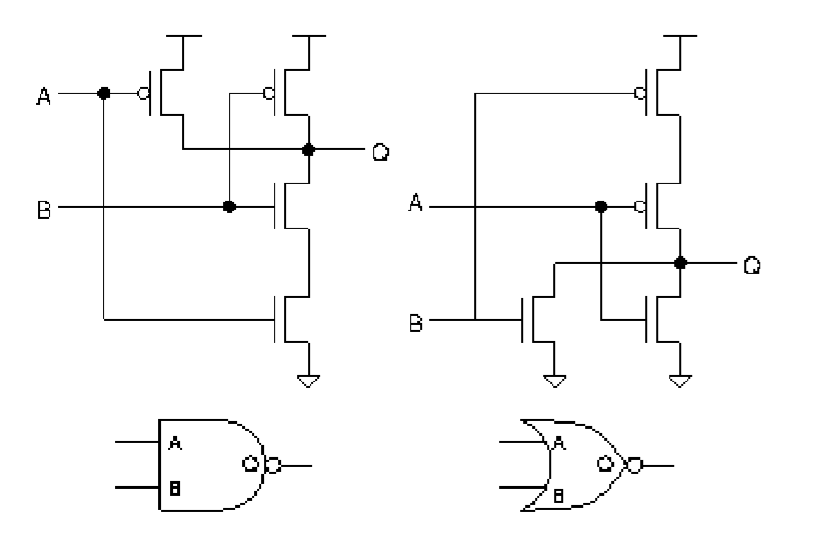
\includegraphics[width=9cm]
		{csa/gates}}
	\caption{\label{fig:gates} NAND and NOR gates}
\end{figure}
If you've done Minecraft Redstone, you might find yourself at home on this section. Sadly real life is a little more complicated.
\paragraph{Combination Logic} A general term for blocks of digital logic which contain no kind of memory. For each $n$ inputs, there are $2^n$ possible output states. Each of these outputs can be represented by a basic boolean algebra (eg. $A\wedge B$) and written into a circuit as such.
\subsection{ALU}
multiplexer
adders/halfadder
flip-flops and latches

\section{Architecture}
\subsection{von Neumann}
\begin{figure}[!htb]
	\center{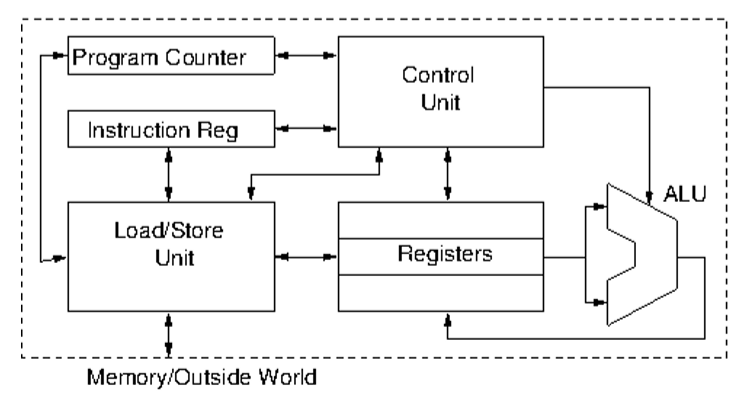
\includegraphics[width=9cm]
		{csa/vonover}}
	\caption{\label{fig:vonover} von Neumann Overview}
\end{figure}
von Neumann architecture is the more common CPU architecture used in modern times. There are a few components, as seen in the figure, and they each serve their unique purpose.
\begin{enumerate}
	\item Main Memory: Logically seperate from the CPU; it holds all the instructions and data that make up a program. This data is stored in distinct locations, referred to as "memory addresses."
	\item Load/Store Unit: The interface between the CPU and the outside world; transfers data via the bus.
	\item Registers: Local, fast storage that holds data currently in use. Each register holds one "word" of data. Does not hold instructions.
	\item Instruction Register: Holds instruction. This is used by the control unit to configure the ALU. In usual design, only one instruction is active at any given time.
	\item ALU: Arithmetic Logic Unit; where computations take place. Reads data from registers and writes results back into registers.
	\item Program Counter: Special register that contains the memory address of the next instruction to execute.
	\item Extra:
	\begin{enumerate}
		\item Cache: Intermediate memory between CPU and Main Memory used for fast access of external memory
		\item IO Controller: Handles peripheral devices via an extension of memory addressing protocol or interrupt-based protocol. Connects via bus.
	\end{enumerate}
\end{enumerate}
memory, load/store unit, registers, instruction register, alu, program counter, 

\subsection{Execution}
\paragraph{Fetch-Decode-Execute}
\begin{enumerate}
	\item Inspect the program counter to find the address of the next instruction
	\item Load the next instruction from memory into the instruction register
	\item Update the program counter to point at the next instruction
	\item Determine the type of instruction fetched
	\item If the instruction requires data from memory, determine its address
	\item Fetch any required data from memory into one of the CPU registers
	\item Execute the instruction
	\item Return to step 1 for next instruction
\end{enumerate}

\section{MIPS Microarchitecture}
This section deals with the MIPS microarchitecture and how to construct it.
\begin{itemize}
	\item Microarchitecture: Detailed structure and organisation of the machine.
	\item Datapath: Collection of functional units which implement the instruction set.
	\item Control Logic: Configures the datapath in the correct way so that it implements the desired instruction.
\end{itemize}
\subsection{Building Datapath}
\paragraph{Instruction Fetch}
The first step of the instruction cycle is to get the address of the next instruction and then fetch the instruction itself. To do this, we must send the contents of the program counter to memory, as an address, and bring the contents of that address into the CPU as the next instruction. We will need the Program Counter, Main Memoru (usually physically off-chip) and an Instruction Register. We will also need an "adder" of sorts to increment the Program Counter. 
\begin{figure}[!htb]
	\center{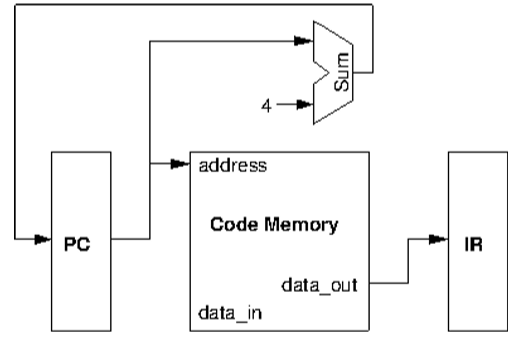
\includegraphics[width=7cm]
		{csa/mipsinstruct}}
	\caption{\label{fig:mips1} Instruction Fetch datapath sketch}
\end{figure}
\paragraph{R-Type Instruction}
R-Type instructions are instructions where all data values used are in the register. Each 32-bit R-Type instruction is partitioned as follows:
\begin{itemize}
	\item 6-bits: Opcode (machinecode representation of the instruction)
	\item 5-bits: Source 1
	\item 5-bits: Source 2
	\item 5-bits: Destination
	\item 5-bits: Shift
	\item 6-bits: Funct (For instructions that share an opcode, the funct parameter contains the necessary control codes to differentiate the different instructions.)
\end{itemize}
As such, 15 of these bits are dedicated to selecting registers that are involved in ALU computations.
\begin{figure}[!htb]
	\center{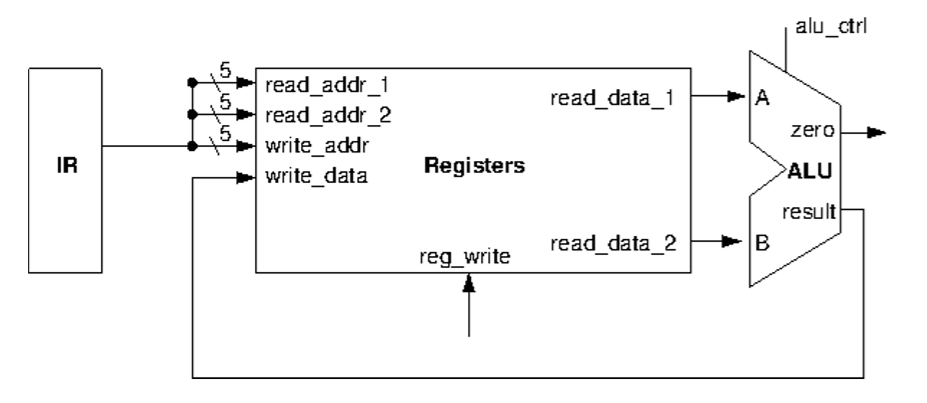
\includegraphics[width=10cm]
		{csa/rtype}}
	\caption{\label{fig:rtype} R-Type instruction datapath}
\end{figure}
\newpage
\paragraph{Load/Store Instruction}
Load/Store Operations are more complex than ALU instructions; they need to have R/W access to registers, memory and be able to use the ALU to calculate addresses.
\begin{itemize}
	\item 6-bits: Opcode
	\item 5-bits: Base Address (Register containing such address)
	\item 5-bits: Source/Destination (Register containing such address)
	\item 16-bits: Address Offset
\end{itemize}
\begin{verbatim}
lw $t0, 8($sp)
\end{verbatim}
In this example, lw is the opcode, \$t0 is the destination, \$sp is the base address, and 8 is the offset.
One thing to note, is that the address offset is 16 bits, but the ALU processes values at 32-bits. Due to how we represent negative values, and the fact we want to be able to offset in the negative, we will need a Sign Extension Unit to increase our offset to 32-bits before moving it to the ALU.
\begin{figure}[!htb]
	\center{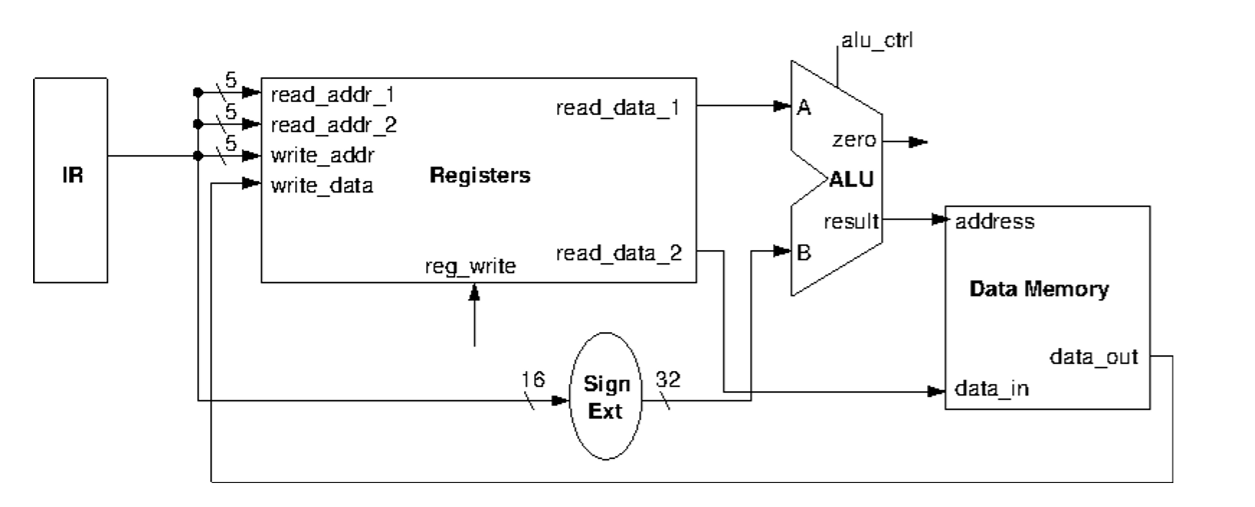
\includegraphics[width=12cm]
		{csa/loadstore}}
	\caption{\label{fig:loadstore} Load/Store Operations Datapath}
\end{figure}
\paragraph{Branches and Jumps}
Branches and jumps essentially achieve the same result; they must both be able to change the contents of the program counter. However, branches require a comparison to be done beforehand, whereas a jump does not. Jumps are a small addition to the structure of a branch datapath, so lets look at branches first.
\begin{itemize}
	\item 6-bits: Opcode
	\item 5-bits: Base Address (Register containing such address)
	\item 5-bits: Source/Destination (Register containing such addres)
	\item 16-bits: Address Offset
\end{itemize}
This is the same instruction structure as Load/Store. However, instead of accessing the memory to, well, load/store, it instead needs to add/increment the PC. This is shown in the diagram.
\begin{figure}[!htb]
	\center{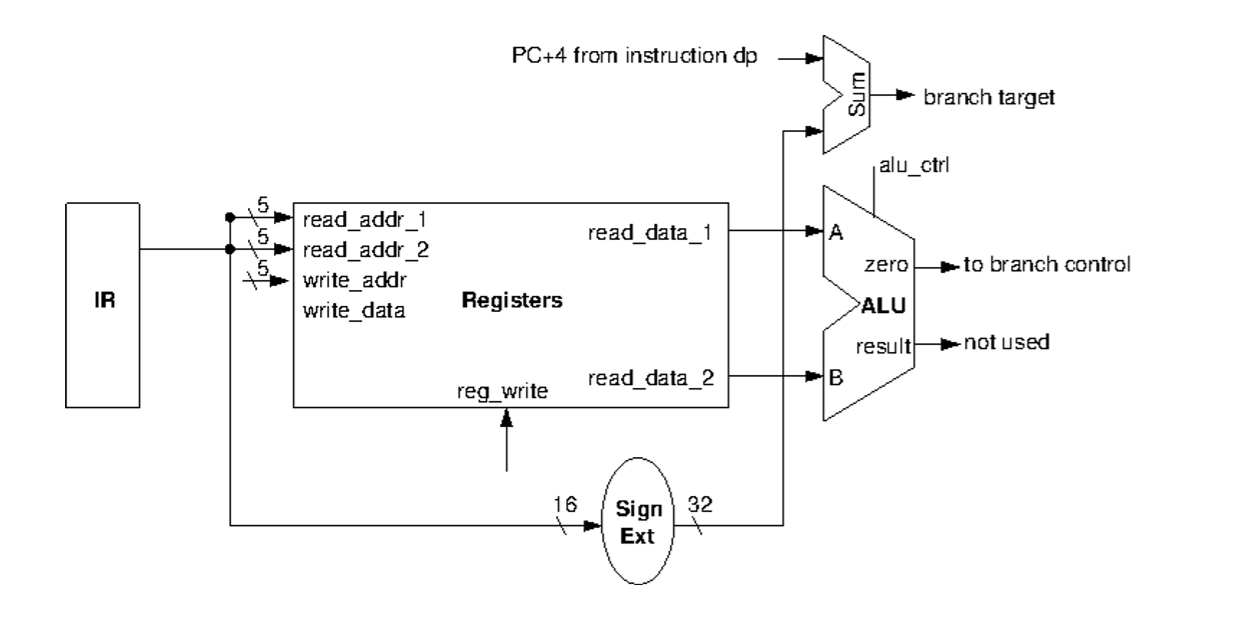
\includegraphics[width=14cm]
		{csa/branch}}
	\caption{\label{fig:branch} Branch Instruction Datapath}
\end{figure}
\paragraph{Combining Datapaths}
instruction fetch (r-type)
load/store (i-type)
multiplexing
integrating them
jump instruction

\section{Optimisation}
\paragraph{Caches}
The cache is a moderately fast, medium-sized memory which acts as a bugger between the main memory component and the registers. Caches are used because of the two basic properties of computer programs.
\begin{enumerate}
	\item Spatial Locality: When an item is referenced, you are likely to access nearby items soon.
	\item Temporal locality: When an item is referenced, you are likely to access it again soon.
\end{enumerate}
At the most fundamental level, cache's are just a block of memory. However, caches need to store a copy of a value from the main memory and its address in the main memory. This address is often called the cache tag. When the CPU is accessing the main memory, it goes through the cache and compares the tag with the address its looking for. It can either hit or miss; because this check is done every time, a cache will add more time than without a cache on a cache miss.
\paragraph{Cache Associativity}
\paragraph{Performance Benefits}

cache
locality
associativity
c/c++ matrices example